\documentclass[twocolumn]{article}

\usepackage{graphicx}
\usepackage{xeCJK}
\usepackage{bm}
\usepackage{amsmath,amsthm,amssymb,amsfonts}
\usepackage{cite}
\usepackage[colorlinks,linkcolor=red,anchorcolor=blue,citecolor=green,CJKbookmarks=true]{hyperref}
\usepackage{indentfirst}
\usepackage{amsmath}
\usepackage[margin=3.5cm]{geometry}
\usepackage{titlesec}
\usepackage{amsmath}
\usepackage{amssymb}
% \linespread{1.6}
\usepackage{multirow}
\usepackage{listings}
\usepackage{xcolor}
\usepackage{ulem}
\geometry{left=1.8cm,right=1.8cm,top=1.5cm,bottom=1.5cm}
\usepackage{enumitem}
\usepackage{tikz}
\usepackage{lipsum}
\setenumerate[1]{itemsep=0pt,partopsep=0pt,parsep=\parskip,topsep=5pt}
\setitemize[1]{itemsep=0pt,partopsep=0pt,parsep=\parskip,topsep=5pt}
\setdescription{itemsep=0pt,partopsep=0pt,parsep=\parskip,topsep=5pt}
%定理
\makeatletter
\thm@headfont{\sc}
\makeatother
\newtheorem{theorem}{Theorem}
%%%%%%%%%%%%% C++ Code
\usepackage{color}
\usepackage{xcolor}
\definecolor{keywordcolor}{rgb}{0.8,0.1,0.5}
\usepackage{listings}
\lstset{breaklines}%这条命令可以让LaTeX自动将长的代码行换行排版
\lstset{extendedchars=false}%这一条命令可以解决代码跨页时,章节标题,页眉等汉字不显示的问题
\lstset{ %用于设置语言为C++
    keywordstyle=\color{keywordcolor} \bfseries, 
    %identifierstyle=,
    basicstyle=\ttfamily, 
    commentstyle=\color{blue} \textit,
    stringstyle=\ttfamily, 
    showstringspaces=false,
    frame=shadowbox, %边框
    %captionpos=b
}

%\setCJKmainfont[BoldFont = 黑体]{宋体}
\setmainfont{Times New Roman}
\setsansfont{Helvetica}
\setmonofont{Courier New}
\setlength{\parindent}{2em}
%如果不要缩进 用\noindent
\title{\LARGE\textbf{Mastering the game of Gomoku with deep \\ neural networks and tree search} \\}

\author{\textbf{Yihong Gu, Yi Xu, Zihan Xu}\\ Tsinghua University \\ \normalsize\ttfamily\selectfont\{gyh15,xuyi15,xzh15\}@mails.tsinghua.edu.cn}

\date{}

\begin{document}

\maketitle

\section{Introduction}

五子棋(Gomoku)是几乎人人都会下的棋类游戏, 如果不设置禁手和相关的限制的话, 黑棋有必胜策略. 因此,我们以五子棋国际比赛使用规则\cite{rule}为蓝本,规定黑棋第一步必须下在棋盘中心,并设置禁手如下:

\begin{itemize}
	\item 黑棋不得下出双活三.
	\item 黑棋不得下出双四.
	\item 黑棋不得下出长连(即超过五个黑子相连).
\end{itemize}

Google在使用AlphaGo战胜Hui Fan后发表的\cite{alphago}的论文中提出了使用deep neural networks和tree search结合的办法来制造围棋AI,其主要思想是使用Monte Carlo tree search的方法,通过神经网络来减少搜索树的深度和宽度.

在\cite{alphago}主要有两种神经网络:policy network和value network. policy network用来模拟行为, value network用来评估胜率.

有四个神经网络,分别是:

\begin{itemize}
	\item \textbf{SL policy network $\bm{p_\sigma}$}:直接用人类专家的棋谱来训练,功能是:给定一个棋局,预测人类会怎么走,目标是提高预测的准确率.
	\item \textbf{fast policy network $\bm{p_\pi}$}:和上述的网络一样,只不过比上述网络训练预测地更快,但是准确度有所下降.
	\item \textbf{RL policy network $\bm{p_\rho}$}:在$p_\sigma$的基础上训练,通过增强学习(reinforcement learning),达到“尽可能地获胜”这个目标(注意这里的目标和$p_\sigma$的不同).功能是:给定一个棋局,返回怎么走最后更有可能赢.
	\item \textbf{value network $\bm{p_\theta}$}:在$p_\rho$的基础上训练,功能是:给定一个棋局,预测如果让$p_\rho$自己和自己下,谁更有可能获胜.
\end{itemize}

在\cite{alphago}的deep neural networks主要是convolutional neural network(卷积神经网络). 在这之前, 卷积神经网络主要被用于图像识别. 可以发现, 围棋的棋感和对图片的整体感知非常像, 一个棋盘可以简单地看成一幅图, 这也是卷积神经网络在AlphaGo的系统中能够表现极好的原因.

五子棋在这一方面和围棋有很多相似的地方, 在我们之前, 在Stanford的CS231n\ref{cs231n}的2016年的Course Project\ref{gomoku}中建立了CNN和RNN(recurrent neural network)的模型, 对于人类五子棋玩家的action进行模拟, 最后达到了将近$40\%$(CNN)和$50\%$(RNN)的准确率, 然而在和五子棋的暴力搜索AI的对决中, 只达到了$0\%$(CNN)和$0.3\%$(RNN)的胜率.

我们用AlphaGo的方法来训练并实现一个五子棋的AI. 同时, 五子棋在训练和AI的实现方面和围棋也有一些区别, 这点在我们之后的实现上也有所体现.

\section{Models}

\subsection{Policy Networks}

\noindent \textbf{Supervised learning of policy networks $\bm{p_\sigma}$, $\bm{p_\pi}$}

在我们机器学习的第一个部分,和\cite{alphago}一样,我们设出假设函数$p_\sigma(a|s)$,表示给定一个棋盘状态$s$,预测人类采取行为$a$的概率.神经网络的输入是一个棋盘状态$s$的一个简单表示(在下一章节中可以看到具体的细节),hidden layer的结构是convolutional layers 和rectifier nonliearities layers相互交替,最后使用softmax分类器算出所有合法走棋$a$的概率分布(distribution).我们最后使用 stochastic gradient descent 来最小化$p_\sigma$和人类玩家对于状态$s$采取的行为$a$之间的cross entropy, 梯度如下

\[
\Delta\sigma \propto \frac{\partial\log p_\sigma(a|s)}{\partial \sigma}
\]

因为黑棋和白棋的走棋有巨大的区别(黑棋有大量禁手),我们对于黑棋和白棋分别训练了一个$8$层的SL policy network. 我们直接选取了RenjuNet\cite{renjunet}数据库中的人类选手比赛数据作为数据集. 在其中的23个规则中,我们选择了在国际比赛中最通用的,也是数据最多的1号规则的数据来训练我们的SL policy network. 数据集中一共有接近60万个合法数据.但是在具体的训练过程中,我们发现在这些数据中, 大多数时候一方在知道必输的情况下会投降, 这样数据集里面几乎没有人类玩家走五子的情况, 为了培养$p_\sigma$的“赢”的意识,我们手动补全了数据.最后的训练中,黑棋的$p_\sigma$达到了$48.5\%$的准确率,白棋的$p_\sigma$达到了$54.1\%$的正确率. 最后的速度是$5$ms一个数据.

我们同时也建立了一个基于用人工设计的feature的linear classifier: fast rollout policy network $p_\pi$,但是他的效果并不是很好,只能到达$20\%$左右的正确率.

\noindent \textbf{Greedy policy oracle}

我们设计的fast rollout policy network $p_\pi$的效果并不好,所以我们使用了AC自动机和人工设计的一些模式,加上部分贪心设计了一个贪心的rollout policy oracle,能够达到$32\%$的正确率,具体的实现细节可以参考下一章节, 由于每一步都需要判断禁手, 禁手的判断时间复杂度很高, 所以最后的速度是0.5ms一个数据.

\noindent \textbf{Reinforcement learning of policy networks $\bm{p_\rho}$}

我们机器学习的第二个部分是RL policy network, 使用policy gradient reinforcement learning训练.神经网络的结构和$p_\sigma$相同并且在一开始使用$p_\sigma$的$\sigma$作为weight的初始值(一开始$\rho = \sigma$).训练中,让当前的神经网络$p_\rho$和他之前的某个版本$p_{\rho'}$打.收益函数(reward function)$r(s)$在$s$为最终结局前($t < T$)都是0,让$z_t=\pm r(s_T)$为最后的回馈,如果这一步是最后赢的人走的,那么$z_t = 1$,否则$z_t = -1$,对于每一步$t$都用 stochasitc gradient descent 来更新,梯度满足

\[
\Delta\rho \propto \frac{\partial\log p_\rho(a_t|s_t)}{\partial \rho}z_t
\]

我们可以感性地从类似于supervised learning的角度理解这个梯度的设计, 如果我这一局赢了, 那么表示在这一局里面我走的每一步都是我值得学习的(即$z_t=1$,可以看成supervised learning); 如果我输了,那么表示在这一局里面我走的每一步都值得我吸取教训(不能这么走,所以朝相反的方向学习即$z_t=-1$). 在具体实现的时候,我们可以类似于supervised learning,赢了的话就是最小化cross entropy,输了的话就是最大化cross entropy.

虽然在\cite{alphago}中未说明,在对走的时候,我们采取随机的方法来提高他的可塑性:即每次先求出$p_\rho$的一个distribution,然后随机一个$[0,1)$随机数,看他落在哪个distribution中,就选择走哪一步.

和$p_\sigma$一样,我们的$p_\rho$也是黑白分开来训练的, 最后我们黑棋和白棋和之前的$p_\sigma$对打都可以达到$80\%$的胜率.

\subsection{Value Networks}

我们需要一个$v_\theta(s)$表示对于棋局$s$,在这个棋局中最后一个落子的那一方赢的概率.这个是很难求的,在实际应用中,我们求近似的$v^p_\theta(s)$表示表示用policy network的策略,对于棋局$s$,预测在这个棋局中最后一个落子的那一方赢的概率,结构和policy network一样仅仅把最后的概率分布改成一个单一的值,目标最小化均方差,从而梯度满足: 

\[
\Delta\theta \propto \frac{\partial v_\theta(s)}{\partial \theta}(z - v_\theta(s))
\]

为了避免overfitting,使用人工数据集,用$p_\sigma$和$p_\rho$随机了300,000个不同的棋局作为数据.

我们尝试了多种参数, 最终由于五子棋过于过于依赖于棋盘局部的状况和近10 - 20步的走棋而不是整体的情况, 所以最后训练的效果并不好, 在数据集足够大的时候只能达到0.8的MSE, 所以我们在最后并没有采用value network.

\section{Implementation of Models}

\subsection{Data Preparation}

在最基础的$p_\sigma$的训练中,我们直接选取了RenjuNet\cite{renjunet}数据库中的人类选手比赛(1号规则)的60万组数据作为数据集. 初步训练完成后, 我们发现在自己亲自和$p_\sigma$对下的时候, $p_\sigma$ 经常已经有了活四却不直接获胜而是去制造更多的活四. 经过仔细研究数据, 我们发现几乎所有的对局都是以一方的投子认输为结束的,所以在这学习过程中$p_\sigma$并没有去学“冲五”, 为了解决这个问题我们手动补全了部分数据.

同时, 大多数数据需要“再走几步”才能让获胜的一方胜利,我们采取了在博弈树上暴力搜索的方法来补全数据,其中主要过程如下:

\begin{itemize}
	\item 连成五子
	\item 选择双三/三四/双四/活四
	\item 选择冲四
	\item 选择活三
\end{itemize}

对于失败的一方,考虑以下策略(优先考虑上面的):

\begin{itemize}
	\item 连成五子
	\item 防对方五子
	\item 防对方双三/三四/双四/活四
\end{itemize}

我们通过搜索博弈树, 如果找到一种获胜的一方获胜的策略,那么就用这个来补全数据.最后这样的方法补全了15647局(其中有1000局左右的平局)中的7119局.

在实际的训练中,对于补全的数据,我们仅仅让$p_\sigma$学习赢的一方赢的策略,对于保守防守的数据,我们没有让$p_\sigma$去学习.

\subsection{Supervised Learning of Policy Networks}

\noindent \textbf{SL policy network $\bm{p_\sigma}$: Architecture}

我们对于白棋和黑棋分别训练policy network

\begin{center}
\makeatletter
\def\@captype{figure}
\makeatother
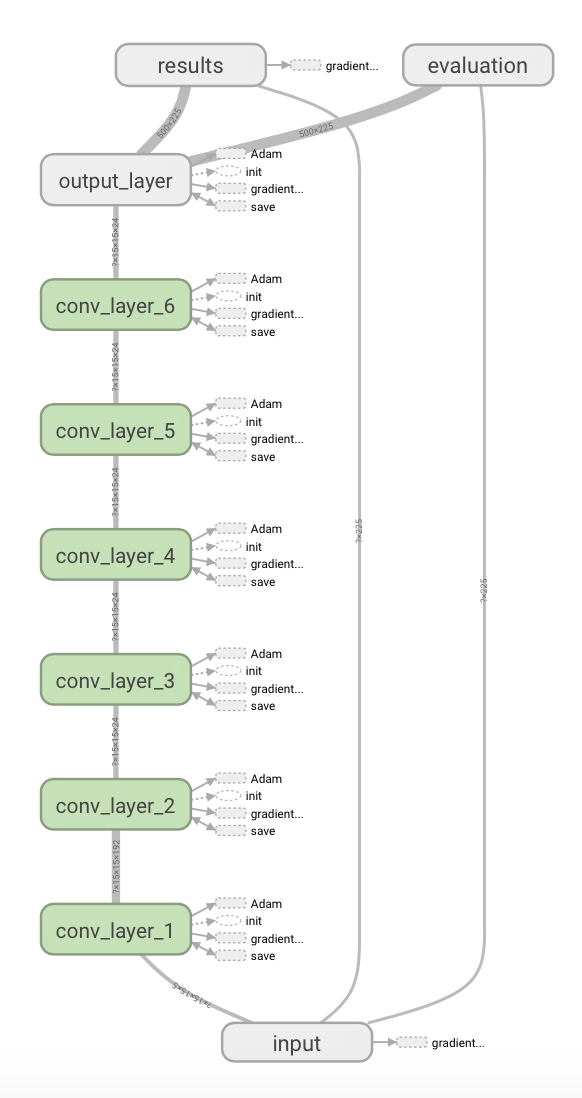
\includegraphics [height=8cm]{network}
\caption{CNN结构}
\label{network}
\end{center}

我们的神经网络的结构如图\ref{network}所示, 一共有8层, 可以看成一个convolutional neural network, 具体各层参数如下: 

\begin{itemize}
	\item \textbf{Input Layer}: $15 \times 15 \times 5$ 的提取的特征, 分为5个slice, 每一个slice是一个$15 \times 15$的矩阵$A$,$a_{i,j}$存储$(i, j)$这个位置的信息, 并且只有0/1两个取值, 5个slice 存储的信息分别是: 全1/全0/是否是我的子/是否是对方的子/是否是空. 这样的特征是非常原始的, 但是由于CNN在特征提取方面的能力, 即使非常原始的特征也能取得比较好的效果. 
	\item \textbf{Hidden Layer 1}: $S = 1$ (Stride), $F = 5$ (Receptive Field), $P = 2$ (Zero Padding), filter: $5 \times 5 \times 5 \times k$,激励函数是relu, 一层的cube是$15 \times 15 \times k$
	\item \textbf{Hidden Layer 2 - 6}: $S = 1$, $F = 3$, $P = 2$, filter: $3 \times 3 \times k' \times k'$(第2层是$3 \times 3 \times k \times k'$),激励函数是relu, 一层的cube是$15 \times 15 \times k'$
	\item \textbf{Output Layer}: 第7层到Output Layer之间的连接用Softmax,$15 \times 15$ 的概率分布.
\end{itemize}

我们尝试了多组$(k, k')$, 最后选择了$k = 81$, $k' = 24$.

\noindent \textbf{SL policy network $\bm{p_\sigma}$: Training}

在训练的时候, 我们黑白分别训练, 把数据集分成训练集, 交叉验证集和测试集三个部分,每个数据包含了输入(棋盘局势$s$)和标记(人类选手的走棋选择$a$). 对于白棋分别是218853(训练集), 60000(交叉验证集), 60000(测试集); 黑棋分别是206701(训练集), 60000(交叉验证集), 60000(测试集).

在训练的时候, 每一步, 随机选择从训练集中选择$m$个样本$\{s^i, a^i\}_{i=1}^m$,使用随机梯度下降法来训练,最小化交叉熵,令梯度为: 

\[
\Delta\sigma = \frac{\alpha}{m} \sum_{i=1}^{m} \frac{\partial\log p_\sigma(a^i|s^i)}{\partial \sigma}
\]

学习速率$\alpha$一开始为$0.003$并且训练$2 \times 10^4$步减少一半, 一共训练了$2 \times 10^5$步,mini-batch size $m = 100$, 最后各自的准确度分别是$54.1\%$(黑)$48.5\%$(白).

\subsection{Greedy Policy Oracle}

由于$\bm{p_\pi}$效果不佳,我们人工设计了一种快速决策的贪心策略(优先考虑上面的):

\begin{itemize}
\item 我方五
\item 防对方五
\item 我方活四/双四/四三
\item 防对方活四/双四/四三
\item 我方双活三
\item 防对方双活三
\item 我方活三或冲四里选同时形成活二最多的一个
\item 我方冲三里同时形成活二最多的一个
\item 其他与在任意一个以已有棋子为中心5*5区域内的形成活二最多的一个
\end{itemize}

这样可以达到$29\%$的准确率.

经过与另一位有写五子棋AI经验的同学的讨论,我们在此基础上进行了一些改进.当然,上面的前六条策略其实是我们必须采用的,因此我们予以了保留.对于剩下的情况,我们采用下面的新方法.

我们将整个棋盘的每个位置用0/1/2表示,1表示我方,2表示对方,那么我们可以用一个0/1/2字符串表示一个五/活四/活三等各种模式,对每种模式设计一个分值.这样,对于一个位置,我们将其所在行/列/两条斜线与这些模式串进行匹配(通过AC自动机实现),将分值和作为对这一位置的评估.由于对一个位置的评估函数那位同学已经实现过了,我们直接对其进行了调用.

在决策的时候,我们只要选取落子后评估增量最大的位置就可以了.

由于分值比之前的数活二个数考虑更为全面细致, 也加入了人的考虑, 使得准确率略有提升,达到了$32\%$.

除此以外, 这样做一个极大的好处是, 对于那些固定策略以外的情况, 我们可以根据评估增量实现按概率分布落子, 方便Monte Carlo tree search中的rollout部分使用.

\subsection{Value Networks}

\noindent \textbf{Value networks $\bm{v_\theta}$: Architecture}

value network $v_\theta$的结构和$p_\sigma$基本一致

\begin{itemize}
	\item \textbf{Input Layer}: $15 \times 15 \times 5$ 的提取的特征, 意义同$p_\sigma$
	\item \textbf{Hidden Layer 1}: $S = 1$ (Stride), $F = 5$ (Receptive Field), $P = 2$ (Zero Padding), filter: $5 \times 5 \times 5 \times k$,激励函数是relu, 一层的cube是$15 \times 15 \times k$
	\item \textbf{Hidden Layer 2 - 6}: $S = 1$, $F = 3$, $P = 2$, filter: $3 \times 3 \times k' \times k'$(第2层是$3 \times 3 \times k \times k'$), 激励函数是relu, 一层的cube是$15 \times 15 \times k'$
	\item \textbf{Hidden Layer 7}: $S = 1$, $F = 1$, $P = 0$, filter: $1 \times 1 \times k \times k'$, 最后在reshape成一个$225$个节点的层, 激励函数是relu. 
	\item \textbf{Hidden Layer 8}: 第7层到第8层是全连接, 激励函数是relu.
	\item \textbf{Output Layer}: 第8层到Output Layer之间的连接用tanh,最后生成一个$[-1,1]$的整数表示己方获胜的概率.
\end{itemize}

\noindent \textbf{Value network $\bm{p_\rho}$: Training}

数据集来自于用$p_\sigma$和$p_\rho$创建的$3 \times 10^5$组人工数据.

对于每个数据,执行以下几步

\begin{itemize}
	\item 随机一个数$U$(1 - 60),前$U-1$步都用$p_\sigma$走. 
	\item 第$U$步随机走(随机找一个合法的). 
	\item 接下来都用$p_\rho$走,一直走到完,算出$z_T$.
	\item 把$(s_{U+1}, z_{U+1})$放入数据集. 
\end{itemize}

最后最小化均方差, 梯度如下:

\[
\Delta\theta = \frac{\alpha}{m} \sum_{i=1}^m\frac{\partial v_\theta(s^i)}{\partial \theta}(z^i - v_\theta(s^i))
\]

我们尝试了多种参数, 在这个只能达到0.8的MSE, 所以我们在最后并没有采用value network.

\section{Tree Search Algorithm}

\subsection{Overview}

我们采用Monte Carlo tree search作为主要算法.

考虑Monte Carlo tree上的每一个点,都表示一个棋局的状态$s$,每条边都可以用$(s, a)$来表示,其中$a$是一个合法的走棋,Monte Carlo tree search的算法分为4个部分.

\noindent\textbf{Selection}: 对于当前的点,如果不是叶子节点,考虑下一步的sampling该选哪一步,基于UCT算法的改良,我们选择$Q(s, a) + u(s, a)$最大的那个,一直往下走到叶子节点$s_L$\textbf{(注意此时这个节点还不在树中,但是这个节点的父亲在树中)}为止.其中$u(s, a) = c_{puct}P(s, a)\frac{\sqrt{\sum_{b}N(s,b)}}{1+N(s,a)}$,$P(s, a)=p_\sigma(a|s)$ 用SL Policy Network $p_\sigma$来算,$N(s,a)$表示$(s,a)$这条边参加sampling的次数.

\noindent\textbf{Evaluation}: 从叶子节点$s_L$开始,接下来用$p_\pi$来模拟双方落子行为,算出最后的输赢情况$z_L$,然后计算出叶子节点在这一轮模拟中的值$V(s_L^i)=(1-\lambda)v_\theta(s_L) + \lambda z_L$.

\noindent\textbf{Backup}: 向上更新所有的祖先的$Q$值和$N$值.其中$N(s, a) = \sum_{i=1}^n[(s,a,i)]$,$Q(s, a) = \frac{1}{N(s,a)}\sum_{i=1}^n{[(s,a,i)] \cdot V(s_L^i)}$,其中$[(s,a,i)]$为$1$当且仅当在第$i$轮模拟中经过了$(s, a)$这条边.

\noindent\textbf{Expansion}: 如果某条边$(s, a)$的访问次数超过了阀值,就把$s'= f(s,a)$加入到搜索树中来,$f(s,a)$表示这个边连向的某个儿子.

在搜索完成之后,我们的AI会选择走$N(s, a)$最大的那个$a$,保留$s'=f(s, a)$子树的内容,然后释放其他所有节点的内存.

\subsection{Implementation Details}

\underline{具体实现中为了加快速度可以使用多线程},在MCTS中的每个节点$s$都包含由\textbf{所有}合法操作$a$组成的边$(s,a)$,对于每条边,都需要记录一下数据:

\begin{itemize}
	\item $P(s, a)$ 即Overview中的$P(s, a)$
	\item $N_v(s, a)$ 即Overview中的$N(s, a)$,这里细化指的是在这棵子树中计算过的$v_\theta(s)$的次数.
	\item $N_r(s, a)$ 即Overview中的$N(s, a)$,这里细化指的是在这棵子树中计算过的rollout的次数.
	\item $W_v(s, a)$ 指的是在这棵子树中计算过的$v_\theta(s)$的和.
	\item $W_r(s, a)$ 指的是在这棵子树中计算过的rollout的$z_L$的和.
\end{itemize}

\noindent\textbf{Selection}

每次从根开始往下搜索,直到走到一个叶子节点为止(设这时候的时间为L),对于所有的$t < L$,令$a_t = argmax_a(Q(s_t, a) + u(s_t, a))$,其中$u(s, a) = c_{puct}P(s, a)\frac{\sqrt{\sum_{b}N(s,b)}}{1+N(s,a)}$,$c_{puct}$是一个参数,最后被定为$5$.

\noindent\textbf{Evaluation}

把叶子节点$s_L$放到队列中计算$v_\theta(s_L)$(这里采用多线程,并且可以加一个记忆化).对于rollout,下棋双方都用$p_\pi$来模拟,也采用多线程放在队列里依次处理.

\noindent\textbf{Backup}

考虑这次模拟对所有树中边的影响,我们分别更新rollout的值$N_r(s, a), W_r(s, a)$和value network的值$N_v(s, a), W_v(s, a)$,最后更新$Q(s, a)$的值

\[
Q(s, a) = (1 - \lambda)\frac{W_v(s,a)}{N_v(s,a)}+\lambda\frac{W_r(s,a)}{N_r(s,a)}
\]

AlphaGo 中 $\lambda=0.5$的时候效果最好, 我们直接采取了$\lambda=1$.

分别考虑rollout和value network的更新

\begin{itemize}
	\item 对rollout更新的时候,每次把某个节点塞到队列里面计算的时候,就把所有相关的$N_r(s,a)$和$W_r(s,a)$进行修改:$N_r(s,a)=N_r(s,a)+n_{vl}$, $W_r(s,a)=W_r(s,a)-n_{vl}$,让他看起来输了$n_{vl}$场防止多次运算,最后计算出来的时候让$N_r(s,a)=N_r(s,a)-n_{vl}+1$, $W_r(s,a)=W_r(s,a)+n_{vl}+z_L$.
	\item 对value network进行更新的时候,算出来之后更新所有相关的边$N_v(s,a)=N_v(s,a)+1$,$W_v(s,a)=W_v(s,a)+v_\theta(s_L)$.
\end{itemize}

这里$n_{vl}$取$3$.

\noindent\textbf{Expansion}

当一条边$(s, a)$的访问次数超过一个阀值$n_{thr}$的时候,就把后续的状态$s'=f(s,a)$加入到树中,把这个节点的所有边都初始化: $N_v(s',a)=N_r(s',a)=0$,$W_v(s',a)=W_r(s',a)=0$, $P(s',a)=p_\sigma(a|s')$,具体计算的时候$P(s',a)=p_\sigma(a|s')$这步运算也采用多线程,一开始先用tree policy来计算$P(s',a)$(tree policy和rollout policy类似,但是拥有更多的特征值),直到$p_\sigma(a|s')$计算完成之后再让$P(s',a)=p_\sigma^\beta(a|s')$,这里softmax temperature被设为$\beta$,$\beta$取$0.67$,$n_{thr}$需要与实际队列的情况相契合.

\section{Optimization}

\subsection{Straits}

我们对各个部分的棋力作了简单评估, 单纯的$p_\sigma$已经能够下赢一般人. 进一步, 我们将最后的MCTS算法和一个普通的基于剪枝的搜索算法进行了比较, 发现了AlphaGo的MCTS算法在应用到五子棋上的时候会存在一些问题.

在接下来的叙述中, 我们使用在Monte Carlo tree中进行的模拟次数$n_{sm}$来衡量搜索算法的搜索力度. 

在一开始$n_{sm}=50$的时候, 我们发现有的时候算法会走一些“昏棋”, 比如对方有活三却仍然不防, 这主要是由于$p_\sigma$对于部分情况缺少学习并且$n_{sm}=50$过于小导致先验概率在最后的选择中起到了决定性的作用, 针对这些情况我们手动调整$n_{sm}=2000$, 在之后的对决中这些问题就几乎不出现了.

但是, 进行了相关改进之后, 仍然几乎不能赢, 我们对各种参数进行跟踪发现相比较搜索算法而言, MCTS在这种时候几乎很少有构思并设局的能力. 具体而言, 我们发现MCTS在大多时候都是在被动防守, 对方的AI却能够布下连环局最终获得胜利, 这种情况是和五子棋与围棋的差别密切相关的: 五子棋决定胜负的关键在于是否能够布下一个局部的“局”在短时间内获胜, 而围棋更注重于全局更需要对全局的整体把握. 为了解决相关的问题, 我们采取了之后的应对策略.

\subsection{Idea}

分析在Monte Carlo tree中的模拟, 由于我们个人电脑计算速度相对而言较慢导致采样的次数很少($n_{sm}=2000$是基本上要花$30$-$50$s), 所以提高采样的样本的质量成为我们优化的关键.

\subsection{Naive Improvement}

在AlphaGo的实现中, 在一个节点完全是新建的(未被模拟)的时候, $u(s, a)$在决策中起到了决定性的作用, AlphaGo的MCTS算法中$u(s, a)$是这样计算的:

\[
u(s, a) = c_{puct}P(s, a)\frac{\sqrt{\sum_{b}N(s,b)}}{1+N(s,a)}
\]

我们发现, 在第一次搜索的时候, 所有的$u(s, a)$都是$0$, 如果是选择最大的话, 我们会直接返回一个初始值, 这虽然只是多算了一个无用信息但是其连锁反应会给我们的采样的信息加入很多噪点, 在采样量较小的情况下会严重误导我们之后为数不多的采样.

针对这种情况, 我们会在第一次采样的时候直接选取$P(s, a)$, 即$p_\sigma(a|s)$最大的那个a.

\subsection{Damping Curve}

我们发现, 相比较围棋的大局观, 五子棋更注重于局部的较量, 重新考虑rollout的过程, 我们发现如果rollout的局数过于多的话, 实际上他的胜负相对于我目前的局面来看其实并没有任何参考价值, 也就是说, 在rollout中, 存在着一些局数较大的噪点, 在现在$n_{sm}$仅仅是$10^3$级别的时候干扰MCTS的判断. 

基于这一点想法, 我们作出猜想: 一个“局”布置的步数不会超过30步. 在这样的猜想下, 我们改进了我们的rollout: 如果rollout的局数超过30步, 直接放弃并不用来更新相关的参数.

基于这一简单猜想和优化, 我们取$n_{sm}=2000$, 在和之前所述的AI的对决中已经基本能够获取胜利, 但是如果取$n_{sm}=1000$仍然无法取胜.

同时, 我们考虑到随着局数的增加, rollout提供的信息的噪音就越大, 所以我们在$z_L$上乘上一个阻尼函数$\gamma(t)$, 其中$t$表示rollout的步数.

\[
V(s_L^i)=(1-\lambda)v_\theta(s_L) +  \gamma(t) \cdot \lambda z_L
\]

我们凭借直觉加上部分参数调整人工构造了函数$\gamma(t)$

\[
\gamma(t) = 
\begin{cases}
\frac{1}{2}(\tanh(\frac{20 - t}{10}) + 1) & 0 \le x \le 20 \cr
\frac{1}{22}(31-t) & 20 < x \le 30 \cr
0 & otherwise 
\end{cases}
\]

其图如下图\ref{plot}

\begin{center}
\makeatletter
\def\@captype{figure}
\makeatother
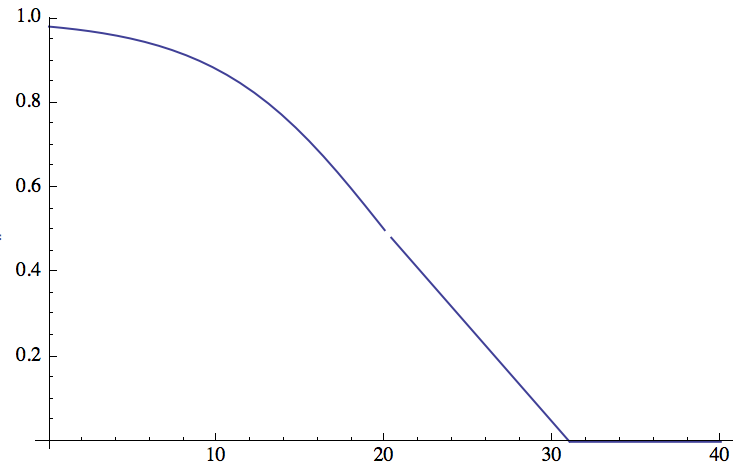
\includegraphics [height=3cm]{plot}
\caption{$\gamma(t)$}
\label{plot}
\end{center}

在这样的优化下, 我们取$n_{sm}=1000$可以获得$50\%$的胜率.

在最后的程序中, 相比较$n_{sm}$, 我们采用更为准确的$n_{rsm}$, 即有效的采样次数(rollout步数小于等于30步的采样的次数)来衡量搜索的力度, 在$n_{rsm}=1000$时对战搜索的AI基本上可以做到稳赢.

同时, 在原来的基础上, 我们用\textbf{非确定步数}来代替原来的\textbf{总步数}, 确定的步包括: 五连, 防对方五连, 三四, 双四, 活四, 这里的确定在于走棋方必然采取这样的策略. 由于在实际对决中经常有通过不断冲四获胜的情况, 所以这样的优化是完全能够起到效果的.

\subsection{Other Differences}

同时, 在先验概率上我们用$p_\rho$代替$p_\sigma$, 在实际测试中能够起到更好的效果.

\section{Conclusion}

考察整个AI系统, 我们发现在实际对战中, $p_\sigma$在搜索的时候给我们提供了一个不错的先验的建议, 实际布局获胜仍然是靠rollout的搜索枚举, 同时相比较暴力搜索, $p_\sigma$的效果也非常明显: 通过先验概率, 我们仅仅只搜索了3万个状态就能战胜搜索了500万个状态的搜索AI. 在把AlphaGo的算法思想移植到五子棋这类更需要“局部设局”的棋类游戏上时, 我们通过神经网络训练的先验概率来提供建议, 同时通过带搜索剪枝的rollout来求得具体的策略, 这是我们整个系统的思路.

\section{Further Work}

我们制作的针对于五子棋的AI仍然有不足的地方, 在之后的实际对战中我们也发现了很多问题. 在之前的总结中, 我们提到了这类AI系统的整体思路: 先验概率提供一个布局的雏形, 让rollout来具体化这个布局. 从这两个角度来看我们有以下的继续优化的空间:

(1) 加快他的采样的速度, 可以进一步记忆化board和rollout, 通过更深入的研究, 我们可以加快判禁手和rollout(贪心)的速度

(2) 增加他的采样的质量, 我们可以对Optimization中提出的damp curve和“不确定步数”作更深入的研究, 同时还可以对先验概率进行优化.

关于对先验概率的优化, 我们结合具体的实践提出了以下几点建议:

\begin{itemize}
	\item 在$p_\sigma$的训练中引入更多slice的feature, 到最后我们才发现, 无论是先验概率的不准确性还是最后局面的难以预测性都是因为$p_\sigma$的训练力度和表达能力还不够.
	\item 我们可以用现在的MCTS+先验概率的结合体来增强学习,增强其先验概率的质量.
\end{itemize}

\section{System Architecture}

整个系统(c++代码)可以分为七个部分,具体如下:

\begin{itemize}
	\item \textbf{Oracle}部分: 主要用来调用神经网络.
	\item \textbf{Player}部分: 玩家类,其中有各种棋类玩家/算法的实现.
	\item \textbf{Board}部分: 棋盘类,其中的\textbf{GomokuBoard}类主要用于棋盘合法性与禁手的判断.
	\item \textbf{Arena}部分: 竞技场类,主要用于$p_\rho$训练中的多次对下迭代和之后对不同玩家/算法的评测.
	\item 信息部分: 存储各种信息\textbf{Move}, \textbf{TreeNode}, \textbf{TreeEdge}
	\item 测试部分: 主要是各种功能的测试, 包括AccuracyCalculator.cpp, ArenaTest.cpp, PlayerpTest.cpp.
	\item 图形化界面部分: 主要实现一个图形化界面.
\end{itemize}

\subsection{Oracle}

Oracle部分包括一个基类\textbf{Oracle}和两个继承类\textbf{pSigmaOracle}和\textbf{pRhoOracle}, 继承关系的UML如图\ref{oracle}

\begin{center}
\makeatletter
\def\@captype{figure}
\makeatother
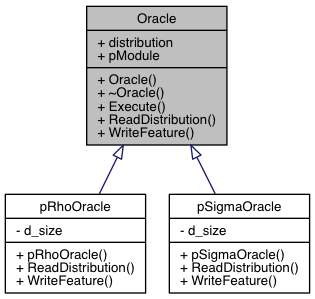
\includegraphics [height=4cm]{oracle}
\caption{Oracle UML继承关系图}
\label{oracle}
\end{center}

Oracle主要负责调用tensorflow对于一个给定的状态$s$求出policy network/value network的概率分布$p(\cdot|s)$,在具体实现的时候,会在c++程序中开一个python虚拟机来实现.

其中各个成员变量的功能如下:

\begin{itemize}
	\item \textbf{pModule}: 用来调用python.
	\item \textbf{distribution}: 用来存储概率分布.
	\item \textbf{d\_size}: 用来存储随机变量的个数(可能是1(value network), 225(policy network)).
\end{itemize}

其中各个成员函数的功能如下:

\begin{itemize}
	\item \textbf{Execute(steps, feature\_file, distribution\_file)}: 在这里使用了多态,给定下棋的步骤steps和存feature的文件名,存distribution的文件名,在这个过程里面会调用python来计算神经网络.
	\item \textbf{WriteFeature(steps, filename)}: 对于不同的子类,按照各自的办法输出feature.
	\item \textbf{ReadDistribution(steps, filename)}: 对于不同的子类,按照各自的办法度入distribution.
\end{itemize}

两个子类的具体说明如下: 

\begin{itemize}
	\item \textbf{pSigmaOracle}: 需要传入子程序的argc, argv[]和python程序的文件名来生成.
	\item \textbf{pRhoOracle}: 需要传入子程序的argc, argv[], python程序的文件名以及tensorflow中存储变量的checkpoint文件的文件名来生成,pRhoOracle会用checkpoint文件中的内容来初始化神经网络,在pSigmaOracle中checkpoint文件的文件名是确定的.
\end{itemize}

\subsection{Player}

Player中是各个玩家/算法的具体实现,其UML图如下图\ref{player}, 继承关系如下图\ref{iplayer}:

\begin{center}
\makeatletter
\def\@captype{figure}
\makeatother
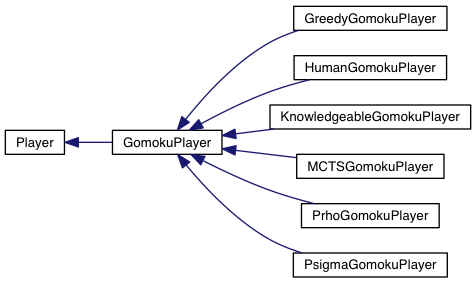
\includegraphics [height=5cm]{iplayer}
\caption{Player 继承关系图}
\label{iplayer}
\end{center}

\begin{center}
\makeatletter
\def\@captype{figure}
\makeatother
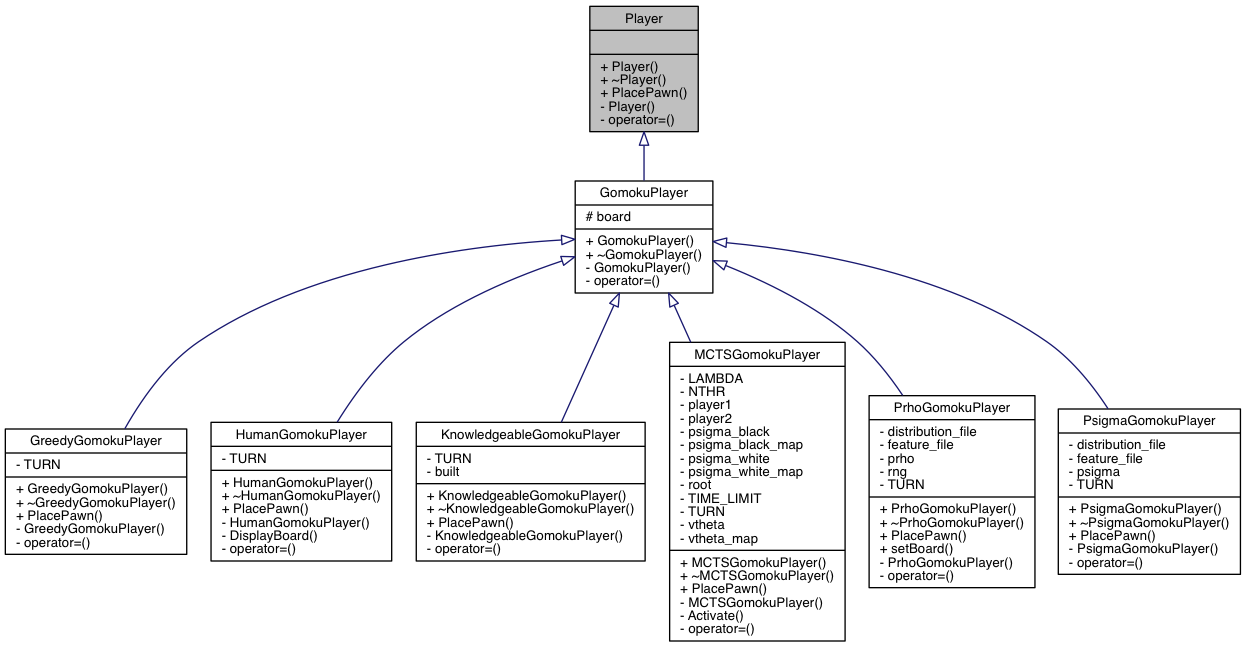
\includegraphics [height=4cm]{player}
\caption{Player UML继承关系图}
\label{player}
\end{center}

\noindent\textbf{Player}类是一个棋类玩家的基类, 有一个虚函数\textbf{PlacePawn()}, 在外界只要调用某一个具体的Player的\textbf{PlacePawn()}函数就可以返回这个玩家的action.

\noindent\textbf{GomokuPlayer}类继承了\textbf{Player}类,并且加入了GomokuBoard的指针能让\textbf{GomokuPlayer}类的子类知道哪些地方不能下.

\noindent\textbf{pSigmaGomokuPlayer}类使用\textbf{pSigmaOracle}来下子,会下$p_\sigma$中合法的概率分布最大的那个

\noindent\textbf{pRhoGomokuPlayer}类使用\textbf{pRhoOracle}来下子,会按照概率分布随机下子(在之前的$p_\rho$训练的时候说过这一点)

\noindent\textbf{GreedyGomokuPlayer}类使用我们最初设计的贪心策略来下子.

\noindent\textbf{KnowledgeableGomokuPlayer}类调用了之前提过的另一位同学的AI.h中的一个位置的评估函数,然后按我们提到的改进策略进行下子.

\noindent\textbf{MCTSGomokuPlayer}类使用前面具体讲解过的MCTS算法进行下子.

\subsection{Arena}

\textbf{Arena}大类的UML继承图如图\ref{arena}

\begin{center}
\makeatletter
\def\@captype{figure}
\makeatother
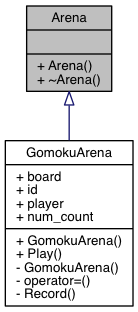
\includegraphics [height=6cm]{arena}
\caption{Arena UML继承关系图}
\label{arena}
\end{center}

\textbf{GomokuArena}类会连接一个\textbf{GomokuBoard}和两个\textbf{GomokuPlayer}的指针,并且会记录这个Arena是第几场(用const变量id和static变量num\_count记录/实现),在用户调用\textbf{Play()}函数来跑的时候会对两个\textbf{GomokuPlayer}进行交互,最后调用\textbf{Record()}函数把棋谱记录在文件中.

\subsection{Board}

我们首先找到了Renlib\cite{renlib}中提供的禁手判断类(CForbiddenPointFinder).由于其本身是为黑棋判断禁手设计,很多函数没有写完整,我们仿照原有代码进行了补充,并添加了一些函数使其更加实用.在此基础上,我们通过继承实现了一个Adapter类Chessboard(后重命名为GomokuBoard), 使其作为其他各类的基本组成部分.继承关系的UML如图\ref{board}.

\begin{center}
\makeatletter
\def\@captype{figure}
\makeatother
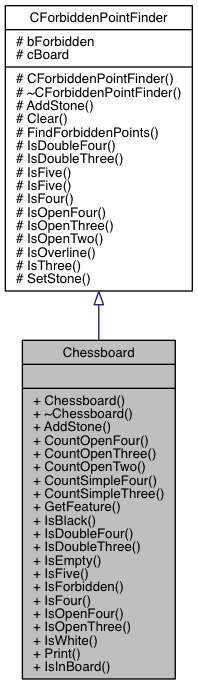
\includegraphics [height=10cm]{board.png}
\caption{Board UML协作图}
\label{board}
\end{center}

\subsection{信息}

信息部分的协作图如图\ref{info}

\begin{center}
\makeatletter
\def\@captype{figure}
\makeatother
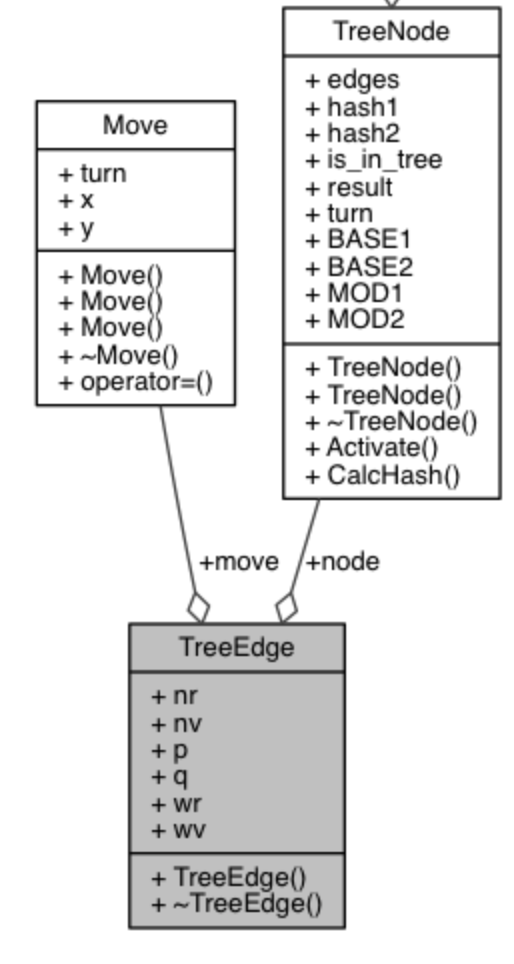
\includegraphics [height=8cm]{info.png}
\caption{信息部分 UML协作图}
\label{info}
\end{center}

\textbf{Move}类存储步的信息,包括下这一步的人是谁以及下的坐标.
\textbf{TreeNode}类存储Monte Carlo tree的结点信息,需要说明的是其中存储了当前棋盘信息的hash值,这样如果已经对于某个棋盘调用过神经网络给出的概率分布,我们就不用再次调用而是直接从map中提取以节省时间.
\textbf{TreeEdge}类存储Monte Carlo tree的边信息.

\subsection{图形界面}

本工程的用户接口,采用了一个开放源代码的围棋图形化演示程序\cite{fff}的修改版本,用于进行五子棋界面的展示、和用户的互动与跨应用程序的通信.该工程使用 Qt 进行编写和设计.为了兼容五子棋的规则和特征,我们修改了该程序以适应五子棋的特征,并基于通用围棋文本传输协议(Go Text Protocal)设计了一个类似的传输协议来对五子棋的棋局数据进行传输.

GUI 程序逻辑控制的主要类为Board类和、Player类.

\textbf{Board} 类为棋盘上棋子的信息,禁手的信息等与棋盘有关的信息提供了存储、访问的通用接口.

\textbf{Player} 类继承自\textbf{QObject},为描述棋局玩家的抽象类,使用中介者设计模式进行架构,为程序主体与玩家、与其他对弈程序之间的互动提供了通用的接口. Player 类包含以下几个重要的成员函数:

\begin{itemize}
	\item \textbf{PlayMove} 成员函数为落子操作提供了通用的接口,通过该函数对落子状态实施通知.
	\item \textbf{Send} 成员函数包装了向该玩家/对弈程序客户端发送指令的过程,通过一个队列来对指令进行存储和发送.
	\item \textbf{GetRespond} 成员函数包装了从该玩家/对弈程序客户端中提取指令的回应的过程,自动提取对指令队列头的指令的回复信息,验证其有效性并对其进行整理.
	\item \textbf{readStandardOutput} 槽包装了从对弈程序客户端的标准输出中提取信息并进行互动的过程.这个函数包装了对不同类型的指令以及相关的回应进行的处理的过程,并包含了游戏过程的主要逻辑.
	\item \textbf{readStandardError}槽包装了从对弈程序客户端的错误输出中提取信息的过程,用于调试与错误信息的显示.
\end{itemize}

此外,控制GUI程序显示的主要类为\textbf{BoardView}和\textbf{Window}类.其中,\textbf{BoardView}为棋盘显示的主要类,负责棋盘的绘制和棋盘信息的显示.\textbf{Window}类为控制主窗口的类,调节主窗口中棋盘显示区域和文字显示区域的关系.

\section{GUI Tutorial}

\subsection{Usage}

使用该 GUI 程序来进行五子棋演示的的使用方式形如 board -gomoku (-black <command> <args>) (-white <command> <args>) 的形式,其中 -gomoku 指定该GUI程序演示五子棋的内容并适用五子棋规则, -black 设定执黑子的程序, -white 设定执白子的程序.若不加以设定,则由人类玩家通过鼠标进行操作.

在没有设定程序的模式下,该 GUI 程序只显示一个棋盘,可以用鼠标进行操作.在设定了对弈程序后,该 GUI 程序将会在界面的左侧展现棋盘画面,右侧展现与对弈程序之间进行的交互有关的信息.在左侧的棋盘画面中,以白色和黑色两色的圈分别代表不同颜色的棋子,以红色的叉形表示黑棋禁止落子的区域.如图 1.png 所示.当鼠标指针移动到棋盘中时,棋盘中的的相应点位将会显示成红色,点击即可在此处落子,如图 2.png 所示.双方轮流进行落子,以第一个达到五个子相连者为胜.

\subsection{Interaction}

该 GUI 程序与对弈程序使用一个基于通用围棋文本传输协议(Go Text Protocal)的一个修改版本的协议进行通信,GUI 程序将会自动调用对弈程序的标准输入输出流来传输与获取数据.该通信协议的主要指令包括以下一些:

\begin{itemize}
	\item play <color> <position> 当前局面下将会在<position>位置下落下<color>颜色的落子.
	\item genmove <color> 以当前局面为背景,生成一步 <color> 颜色的落子.返回落子的位置.
	\item bannedpoint 返回包含所有禁止落子的位置的向量.
	\item showboard 返回当前的棋局状态.
	\item quit 退出程序.
\end{itemize}


下图\ref{g1}是几个效果

\begin{center}
\makeatletter
\def\@captype{figure}
\makeatother
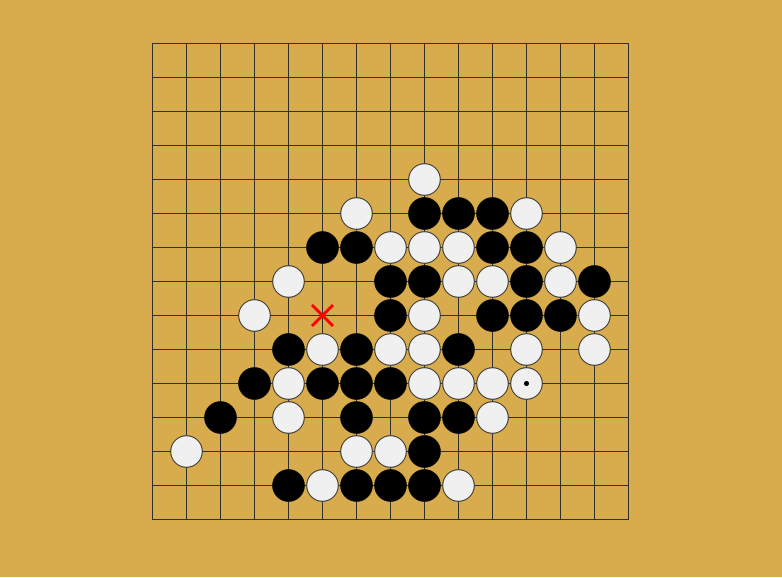
\includegraphics [height=5cm]{1.png}
\caption{GUI界面}
\label{g1}
\end{center}


\begin{thebibliography}{1}
\bibitem{alphago}
Silver, David, et al. Mastering the game of Go with deep neural networks and tree search, Nature 529.7587: 484-489, 2016
\bibitem{cs231n}
Stanford University CS231n: Convolutional Neural Networks for Visual Recognition, http://cs231n.stanford.edu/project.html, 2016
\bibitem{gomoku}
Rongxiao Zhang, Convolutional and Recurrent Neural Network for Gomoku, Course Project of CS231n, 2016
\bibitem{rule}
http://www.renju.net/study/rules.php, 2016
\bibitem{renjunet}
http://www.renju.net/downloads/games.php, 2016
\bibitem{fff}
https://github.com/Mezoka/Board
\bibitem{renlib}
http://www.renju.se/renlib/opensrc/
\end{thebibliography}

\end{document}

